\documentclass[11pt,a4paper]{article}
\usepackage[T1]{fontenc}
\usepackage[utf8]{inputenc}
\usepackage{lmodern,microtype}
\usepackage{geometry}
\geometry{margin=23mm,headheight=14pt}
\usepackage{setspace}
\setstretch{1.08}
\usepackage{booktabs,array,tabularx}
\usepackage{amsmath,amssymb}
\usepackage{graphicx,xcolor}
\usepackage{tikz}
\usetikzlibrary{arrows.meta,positioning,calc}
\usepackage{pgfplots}
\pgfplotsset{compat=1.18}
\usepackage{caption,hyperref,fancyhdr}
\hypersetup{colorlinks=true,linkcolor=blue!55!black,citecolor=blue!55!black,urlcolor=blue!55!black,pdftitle={The Economics of an Indigenous Optimization Solver for India}}
\pagestyle{fancy}
\fancyhf{}
\fancyhead[L]{\small Indigenous Optimization Solver: India Cost Analysis}
\fancyfoot[C]{\thepage}
\setlength{\parskip}{0.36em}
\setlength{\parindent}{0pt}
\newcommand{\inr}{\ifmmode\text{INR}\,\else INR\,\fi}
\newcommand{\lac}{\ifmmode\,\text{lakh}\else\,lakh\fi}
\newcommand{\crr}{\ifmmode\,\text{crore}\else\,crore\fi}

\begin{document}
\begin{center}
{\LARGE\bfseries The Economics of an Indigenous Optimization Solver for India\par}
\vspace{5pt}
{\large A bottom-up market boundary, cost model, and adoption analysis for SIH26119\par}
\end{center}
\vspace{6pt}

\begin{abstract}
Problem statement SIH26119 calls for an indigenous LP, MILP, and QP solver core that can be examined and adapted for Indian industrial applications. Its potential value is strategic, but a software capability does not by itself establish a saleable market or an economic saving. This paper constructs a reproducible, bottom-up INR scenario from Indian government enterprise and refinery counts. It separates documented organization counts from assumed model suitability, contract value, adoption, and engineering cost. The Department of Public Enterprises reports 291 operating central public sector enterprises (CPSEs) in FY2024--25, including 97 in manufacturing, processing, and generation. Six refinery CPSEs within that sector form a narrow initial account list. At an assumed \inr10\lac{} annual contract value, these imply a gross 291-account ceiling of \inr29.1\crr{}, a scenario-based serviceable sector opportunity of \inr2.4--7.3\crr{}, and a conditional first-year revenue scenario of \inr10--30\lac{} from one to three paid pilots. None is a measured software market, signed order, realized SOM, or forecast. An illustrative \inr60\lac{} annual fixed cash budget plus \inr3\lac{} direct cost per account requires nine annual \inr10\lac{} contracts to cover ongoing cash costs. The six-refiner beachhead alone cannot do so. The commercial case depends on demonstrated model performance, customer validation, a larger qualified account list, and actual procurement evidence.
\end{abstract}

\section{Decision question and scope}

The proposed product is an optimization \emph{engine}: it takes a mathematical model and returns a checked solution, a bound or gap where appropriate, and diagnostic status. The SIH26119 statement asks for LP, MILP, and QP support, sparse and numerically robust computation, an API or CLI, recognized benchmarks, and GPU acceleration where it demonstrably helps. It does not specify a monetary license target or a scoring threshold. The project has a substantial local implementation and public benchmark records, but no MRPL operating-data validation, signed customer contracts, or measured buyer willingness to pay in the supplied folder.\footnote{Project evidence inspected for this paper includes \texttt{SIH-backup-solver/Problem Statement.txt}, \texttt{reports/milp-iteration-37/REPORT.md}, \texttt{docs/V2\_LIMITATIONS.md}, and \texttt{reports/KAGGLE\_GPU\_REPORT.md}. Historical benchmark results concern their identified binaries and settings; they are not commercial revenue data.}

This paper asks three narrower questions. First, what countable Indian organizations could reasonably \emph{begin} a market assessment? Second, what annual cash budget and customer contribution would sustain a small engineering team? Third, what evidence must be obtained before a buyer can claim operational value or a vendor can claim that an addressable account will pay? These questions matter even if the solver remains a government-funded research asset rather than a commercial service.

All financial figures below are nominal INR and exclude GST, income tax, financing charges, inflation, bad debt, and discounting. Market counts are historical observations from dated sources; monetary inputs are clearly marked \emph{scenario assumptions}. Revenue is annual recurring contract value (ACV), which could include maintenance, support, and restricted deployment services. The report does not assume a particular intellectual-property or open-source license for the team's code.

\section{Evidence ledger and accounting unit}

\begin{table}[htbp]
\centering
\caption{What is sourced and what remains hypothetical. A site, a legal organization, and a purchase contract are different units.}
\label{tab:evidence}
\small
\begin{tabularx}{\textwidth}{@{}p{35mm}p{34mm}X@{}}
\toprule
Item & Basis & Meaning and boundary\\
\midrule
291 operating CPSEs & DPE Public Enterprises Survey, FY2024--25 \cite{dpe2025} & Observed legal-enterprise universe across all sectors. Some may have no need for optimization software. Not an estimate of buyers.\\
97 manufacturing, processing, and generation CPSEs & Same DPE survey \cite{dpe2025} & Observed subset of 291. Includes refining and power activities. Sector membership alone does not demonstrate a model, budget, or procurement path.\\
23 positive-capacity PPAC facility rows & PPAC capacity table, 1 April 2026 \cite{ppac2026} & Inference: 24 listed rows minus one zero-capacity Cauvery Basin row. This does not establish 23 operating sites; HRRL was scheduled to begin commercial operation only later in 2026 \cite{hrrl2026}. Sites are not distinct buyers.\\
Six sector refinery CPSEs & DPE Appendix II \cite{dpeappendix} & Initial organization-level account list: BPCL, CPCL, HPCL, IOCL, MRPL, and NRL. Subsidiary or centralized procurement could mean fewer independent contracts. ONGC belongs to the mining sector, outside this nested subset.\\
1--3 prospective paid pilots & Team first-year scenario & A conditional adoption target. Realized SOM is unverified: no signed agreement, procurement approval, or price discovery was supplied.\\
Contract value and costs & Team scenario & \inr5--15\lac{} ACV sensitivity, \inr60\lac{} annual fixed cash cost, and \inr3\lac{} direct annual cost per customer. They are budget assumptions, not invoices or quotes.\\
\bottomrule
\end{tabularx}
\end{table}

The Department of Public Enterprises (DPE) classifies 291 operating CPSEs in FY2024--25, 97 of them in manufacturing, processing, and generation \cite{dpe2025}. This creates a useful \emph{account universe} for screening. It cannot be translated into an optimization software market by multiplying every enterprise by an invented price. MoSPI's 2023--24 Annual Survey of Industries landing page reports about 2.6 lakh estimated factories in total; the detailed results identify 2,12,990 registered factories in operation \cite{asi2024,asisummary}. These are facilities, not software-purchasing legal entities, and many will never buy a general optimization engine. Consequently those larger statistics appear only as industrial context, not in the revenue calculation.

PPAC's 1 April 2026 capacity table contains 24 listed facility rows and one zero-capacity Cauvery Basin row, yielding 23 \emph{positive-capacity entries} by direct count \cite{ppac2026}. Positive listed capacity does not establish operation on that date: an April 2026 government release still described HPCL Rajasthan Refinery Limited (HRRL) as a project with a scheduled commercial operation date of 1 July 2026 \cite{hrrl2026}. We therefore make no operating-site count from the PPAC table. DPE Appendix II identifies exactly six operating petroleum refinery/marketing CPSEs inside its 97-company manufacturing, processing, and generation sector: BPCL, CPCL, HPCL, IOCL, MRPL, and NRL \cite{dpeappendix}. ONGC is classified in crude-oil mining and is a possible \emph{cross-sector} lead; adding it to this sector's beachhead would break the nested funnel. Parent/subsidiary procurement may reduce the number of independently paying entities below six.

\section{A nested market funnel, not a published market size}

\subsection{Definitions and formulas}

We use three explicit levels. \emph{TAM ceiling} is a broad hypothetical public-sector account envelope, not the value of India's full solver market. \emph{SAM} is the part of a relevant DPE sector assumed to have a suitable model and procurement potential. \emph{Prospective SOM} is a conditional target of paying pilot organizations in a first commercial year; realized SOM is unverified. The six-refinery account list is a beachhead between the SAM and prospective SOM levels. These sets are nested in the accounting model; they must not be summed.

Let \(A\) be assumed annual contract value in lakh rupees, \(q\) the unknown share of the 97 sector CPSEs passing \emph{technical, model-access, budget, and procurement} qualification, and \(n\) the number of prospectively paying pilots. We compute
\begin{align}
T_{\mathrm{ceiling}}(A) &= 291A/100 \quad\text{crore INR per year}, \label{eq:tam}\\
S_{\mathrm{sector}}(A,q) &= \left\lfloor97q+\tfrac12\right\rfloor A/100
   \quad\text{crore INR per year},\label{eq:sam}\\
B_{\mathrm{refinery}}(A) &= 6A \quad\text{lakh INR per year},\\
O_{\mathrm{pilots}}(A,n) &= nA \quad\text{lakh INR per year}. \label{eq:som}
\end{align}
The factor 100 converts lakh to crore. There is no measured \(q\) or \(A\), so every monetary output is a conditional calculation. For reporting, \(\lfloor97q+\tfrac12\rfloor\) rounds nonnegative account counts to the nearest integer with halves rounded upward; thus \(97(0.50)=48.5\) becomes 49. This is arithmetic rounding, not a survey result. Because \(q\) bundles model fit and purchasing eligibility, this SAM is a \emph{scenario proxy}, not a verified serviceable market.

\begin{figure}[htbp]
\centering
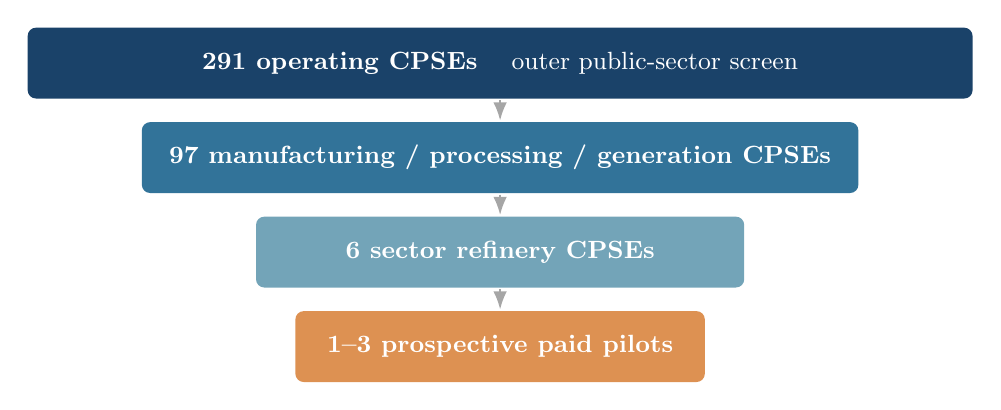
\begin{tikzpicture}[font=\small,>=Latex]
  \definecolor{deep}{RGB}{26,66,105}
  \definecolor{mid}{RGB}{50,115,153}
  \definecolor{pale}{RGB}{115,164,184}
  \definecolor{warm}{RGB}{221,145,82}
  \fill[deep,rounded corners=3pt] (-6,0) rectangle (6,0.9);
  \node[text=white,align=center] at (0,0.45)
  {\textbf{291 operating CPSEs} \quad outer public-sector screen};
  \fill[mid,rounded corners=3pt] (-4.55,-1.2) rectangle (4.55,-0.3);
  \node[text=white,align=center] at (0,-0.75)
  {\textbf{97 manufacturing / processing / generation CPSEs}};
  \fill[pale,rounded corners=3pt] (-3.1,-2.4) rectangle (3.1,-1.5);
  \node[text=white,align=center] at (0,-1.95)
  {\textbf{6 sector refinery CPSEs}};
  \fill[warm,rounded corners=3pt] (-2.6,-3.6) rectangle (2.6,-2.7);
  \node[text=white,align=center] at (0,-3.15)
  {\textbf{1--3 prospective paid pilots}};
  \draw[->,gray!70,line width=.8pt] (0,-.02)--(0,-.28);
  \draw[->,gray!70,line width=.8pt] (0,-1.22)--(0,-1.48);
  \draw[->,gray!70,line width=.8pt] (0,-2.42)--(0,-2.68);
\end{tikzpicture}
\caption{Account funnel. DPE supplies the first three nested enterprise counts \cite{dpe2025,dpeappendix}; the last range is a conditional adoption assumption, not realized SOM. Width is illustrative and does not represent revenue share.}
\label{fig:funnel}
\end{figure}

\subsection{Illustrative INR opportunity}

Table~\ref{tab:market} fixes \(A=\inr10\lac\) and varies suitability \(q\). The full 291-account multiplication is useful only as an upper screen. A serviceable opportunity requires model-level and procurement-level qualification; the six-refinery beachhead would be smaller still. ONGC, private refineries, state utilities, logistics firms, and private manufacturers are excluded from this sector-specific beachhead calculation, not declared to have zero potential.

\begin{table}[htbp]
\centering
\caption{Illustrative annual contract-value scenarios at assumed \inr10\lac{} ACV. Counts of suitable accounts and all INR totals are estimates, not actual customers or sales.}
\label{tab:market}
\small
\begin{tabularx}{\textwidth}{@{}p{40mm}p{34mm}p{31mm}X@{}}
\toprule
Level & Account arithmetic & Annual INR & Interpretation\\
\midrule
Outer CPSE ceiling & \(291\times 10\lac\) & \inr29.1\crr & All 291 buy; intentionally unrealistic upper screen.\\
Sector SAM, low & \(\lfloor97(0.25)+0.5\rfloor=24\) & \inr2.4\crr & 25\% qualifying-share assumption.\\
Sector SAM, central & \(\lfloor97(0.50)+0.5\rfloor=49\) & \inr4.9\crr & 50\% qualifying-share assumption.\\
Sector SAM, high & \(\lfloor97(0.75)+0.5\rfloor=73\) & \inr7.3\crr & 75\% qualifying-share assumption.\\
Refinery beachhead ceiling & \(6\times10\lac\) & \inr60\lac & Every sector refinery CPSE buys separately.\\
Prospective SOM scenario & \((1\text{ to }3)\times10\lac\) & \inr10--30\lac & Conditional paid-pilot target; realized SOM unverified.\\
\bottomrule
\end{tabularx}
\end{table}

The assumed contract value is itself a dominant uncertainty. At \inr5, \inr10, and \inr15\lac{} ACV, the 291-account arithmetic ceiling is respectively \inr14.55, \inr29.10, and \inr43.65\crr{}. For the 49-account central sector screen it is \inr2.45, \inr4.90, and \inr7.35\crr{}. Those are \emph{possible invoice totals under assumptions}, not a market research estimate. A future buyer survey should ask whether an optimization problem is recurring, whether it has a current solver or manual workaround, model sizes and accuracy requirements, who owns the budget, and the cost of switching.

\subsection{Why an account may drop out}

An enterprise belongs in a serviceable count only after all of the following are demonstrated:
\begin{enumerate}
  \item It has at least one recurring LP, MILP, or convex-QP planning decision, with a model that may be used for evaluation.
  \item The product solves that model within agreed time, feasibility, and objective-gap criteria, including difficult and perturbed instances.
  \item Data-security, infrastructure, procurement, and intellectual-property terms permit a pilot.
  \item There is an economic owner who accepts a priced proposal after comparing feasible alternatives.
\end{enumerate}
The observed DPE count establishes none of these four tests. Conversely, a single parent company may operate several refineries but sign one master contract. Thus PPAC's 23 positive-capacity facility entries cannot be added to DPE's 291 companies or to the six-CPSE shortlist. The national all-sector TAM also cannot be estimated from the present evidence: no India-wide count of solver-buying organizations or transaction prices was found in the project files.

\section{Competitive price evidence and the value proposition}

\begin{table}[htbp]
\centering
\caption{Publicly checkable comparison. The listed IBM price is development-only; deployment savings cannot be inferred from it.}
\label{tab:competitors}
\small
\begin{tabularx}{\textwidth}{@{}p{30mm}p{47mm}X@{}}
\toprule
Alternative & Verified public pricing or license term & Cost-analysis implication\\
\midrule
IBM ILOG CPLEX & Developer Subscription starts at USD 320 per authorized user per month; IBM says it is for development, not large-scale deployment. Server/cloud deployment pricing requires contact with IBM \cite{ibmprice}. & At an illustrative \inr90/USD conversion, the developer seat costs \inr28{,}800 per month or \inr3.456\lac{} per year before tax. It is \emph{not} a replacement cost for a refinery deployment.\\
Gurobi & Commercial plans depend on deployment, concurrency, and authorized users; a price quote is requested \cite{gurobiprice}. & No defensible India enterprise price or annual savings figure without a buyer-specific quote.\\
HiGHS & Freely available open-source solver under the MIT license \cite{highs}. & License fee may be zero; integration, compute, support, and model validation still cost money.\\
SCIP & Apache 2.0 since version 8.0.3; build dependencies can carry additional license terms \cite{scip}. & Another serious no-fee competitor. A sovereign product cannot claim uniqueness merely because source is inspectable.\\
This project & Proposed \inr5--15\lac{} ACV range in this study. & \emph{Assumed price}, not a market quote or approved product plan. Differentiation requires measured reliability and India-specific stewardship/support.\\
\bottomrule
\end{tabularx}
\end{table}

The SIH statement motivates an inspectable domestic solver core. Domestic stewardship could be valuable for a public industrial customer that wants code audit, local maintenance, on-premises execution, and control over future priorities. Those benefits should be tested in procurement and security review. Free, inspectable HiGHS and SCIP make the competitive question more demanding: the team must demonstrate a reason to adopt \emph{this} engine rather than deploy and support an existing open-source solver. Vendor license savings should not be asserted against HiGHS or SCIP, and a CPLEX or Gurobi deployment saving should not be calculated before obtaining comparable India deployment quotes.

The IBM developer subscription can illustrate only the price of one licensed development seat. USD \(320\times12=\) USD 3,840 annually, or \inr3.456\lac{} at the expressly assumed \inr90/USD conversion. Currency, local taxes, promotional terms, and country availability may vary; the conversion is a scenario input, not an official exchange-rate observation. IBM's own page says commercial deployment pricing is quote-based \cite{ibmprice}. No current client use, renewal, or volume discount can be inferred.

\section{Proposed delivery and annual cash-cost model}

\subsection{Service boundary}

The modelled first offering is a paid technical pilot followed by annual maintenance and support for a validated deployment. It assumes source and executable access can be governed by an agreement; ownership and license terms are unresolved and must be settled before sales. The customer's optimization formulation and data remain its own. An API/CLI engine is sufficient to begin a pilot; a commercial offer additionally needs versioned releases, incident response, security review, regression testing, numerical audit trails, and supported installation.

GPU hardware is not a prerequisite for every model. The project uses local CPU evaluation and separate GPU tests where applicable; the cost model budgets general test compute rather than an always-on GPU server. Kaggle research capacity is not a production hosting contract. There is no measured per-solve electricity bill or verified production workload from which to infer operating energy savings.

\subsection{Fixed and variable cash costs}

Table~\ref{tab:fixed} gives a \emph{planning budget}, not the team's incurred expenditure or a vendor quote. Salaries represent fully loaded annual cash compensation assumptions. Equipment is modelled as an annual lease/support outflow, avoiding a mixture of depreciation and cashflow accounting. The \inr3\lac{} contingency is treated as spent or committed each year in the conservative cash illustration; unused reserve would improve cash. A separate assumed \inr5\lac{} setup outflow appears in the three-year illustration.

\begin{table}[htbp]
\centering
\caption{Illustrative annual fixed cash operating budget (INR lakh). Each row is an assumption, subject to actual staffing and supplier quotes.}
\label{tab:fixed}
\small
\begin{tabularx}{\textwidth}{@{}XrX@{}}
\toprule
Cash item & INR lakh/year & Included work\\
\midrule
Solver engineering, one full-time role & 22 & LP/MILP/QP algorithm maintenance, sparse/numerical fixes, release work\\
Validation and benchmarking, one full-time role & 16 & Reproducible corpus, independent checking, regression and performance tests\\
Domain, security, and deployment support, part-time equivalent & 10 & Model review, data controls, incident and installation design\\
CPU/GPU test compute and storage & 4 & Metered experiments and retained artifacts; no production GPU cluster\\
Equipment lease and hardware support & 2 & Developer/benchmark hosts, repairs, replacement allowance\\
Tools, administration, and secure backup & 3 & Build distribution, logging, access and routine administration\\
Contingency reserve & 3 & Small timing and vendor-cost variability\\
\midrule
\textbf{Annual fixed cash budget \(F\)} & \textbf{60} & \textbf{Scenario total}\\
\bottomrule
\end{tabularx}
\end{table}

Direct delivery cost \(v=\inr3\lac{}\) per annual customer is a further assumption: \inr1.5\lac{} for model onboarding and integration, \inr1.0\lac{} for dedicated support, and \inr0.5\lac{} for deployment monitoring. This cost must be re-estimated from a real pilot; several bespoke refinery models could require much more work. At \inr10\lac{} ACV, annual contribution is \inr7\lac{} per account before fixed cost. Gross contribution margin in this scenario is 70\%, not an observed company margin.

\begin{figure}[htbp]
\centering
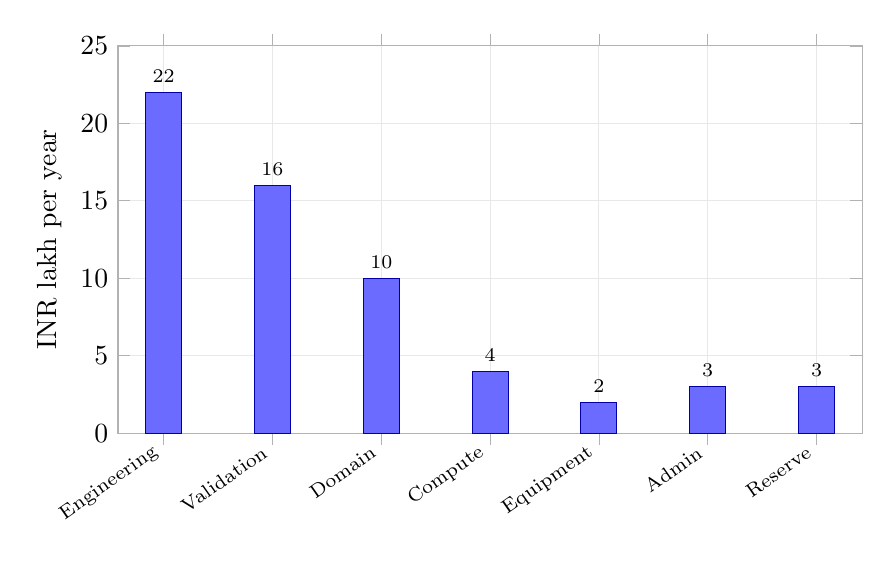
\begin{tikzpicture}
\begin{axis}[
  ybar,bar width=13pt,width=.91\textwidth,height=65mm,
  ymin=0,ymax=25,ytick={0,5,...,25},
  ylabel={INR lakh per year},
  symbolic x coords={Engineering,Validation,Domain,Compute,Equipment,Admin,Reserve},
  xtick=data,x tick label style={rotate=35,anchor=east,font=\scriptsize},
  nodes near coords,nodes near coords style={font=\scriptsize},
  enlarge x limits=.07,grid=major,grid style={gray!18},
  axis line style={gray!60},tick style={gray!60},
  ]
\addplot[fill=blue!58,draw=blue!65!black]
coordinates {(Engineering,22) (Validation,16) (Domain,10) (Compute,4) (Equipment,2) (Admin,3) (Reserve,3)};
\end{axis}
\end{tikzpicture}
\caption{Composition of the assumed \inr60\lac{} annual fixed cash budget; authored from Table~\ref{tab:fixed}, not vendor price data.}
\label{fig:fixedcost}
\end{figure}

\subsection{Buyer-side total cost}

The seller's direct cost is not the buyer's total cost. As a separate illustration, suppose an adopter pays \inr10\lac{} per year for support/deployment and spends \inr4\lac{} internally during the first year of integration, then \inr2\lac{} per year on internal operation and compute in years 2 and 3 only. The three-year undiscounted buyer outflow is
\[
C_{\mathrm{buyer},3}
=3(10)+4+2(2)=\inr38\lac.
\]
These internal costs are unmeasured assumptions. A buyer may need additional migration, validation, security, or training spend. The appropriate value test is whether the candidate produces \emph{validated incremental decision value} exceeding these costs and risks on the customer's own workload. The team has not measured a refinery profit uplift or signed a production service-level agreement. Neither an optimization objective improvement in a teaching example nor a faster public benchmark can be converted directly to rupees of MRPL savings.

\section{Unit economics, break-even, and sensitivity}

For \(N\) paying organizations, annual ACV \(P\) (lakh INR), per-account direct cash cost \(v\), and annual fixed cash cost \(F\), operating cash before tax is
\begin{equation}
\Pi(N,P)=N(P-v)-F,\qquad
N_{\mathrm{break-even}}=\left\lceil\frac{F}{P-v}\right\rceil
\quad(P>v).
\label{eq:breakeven}
\end{equation}
With \(F=60\), \(v=3\), and \(P=10\), the threshold is \(\lceil60/7\rceil=9\) contracts. This is greater than the six-account public-refinery beachhead. Even if every named refinery CPSE bought separately, six contracts would contribute only \inr42\lac{} and leave an \inr18\lac{} annual operating shortfall under these assumptions. This does not mean the project is uneconomic; it means the \emph{assumed} cost and price require expansion, a higher price, lower cost, or noncommercial funding.

\begin{table}[htbp]
\centering
\caption{Break-even sensitivity at \(F=\inr60\lac{}\) and \(v=\inr3\lac{}\) per account per year. Prices are unvalidated assumptions.}
\label{tab:break}
\small
\begin{tabular}{@{}rrrr@{}}
\toprule
ACV \(P\) (INR lakh) & Contribution \(P-v\) (INR lakh) & Required accounts & Six-refinery result\\
\midrule
5 & 2 & 30 & \(-\inr48\lac\)\\
8 & 5 & 12 & \(-\inr30\lac\)\\
10 & 7 & 9 & \(-\inr18\lac\)\\
12 & 9 & 7 & \(-\inr6\lac\)\\
15 & 12 & 5 & \(+\inr12\lac\)\\
\bottomrule
\end{tabular}
\end{table}

\begin{figure}[htbp]
\centering
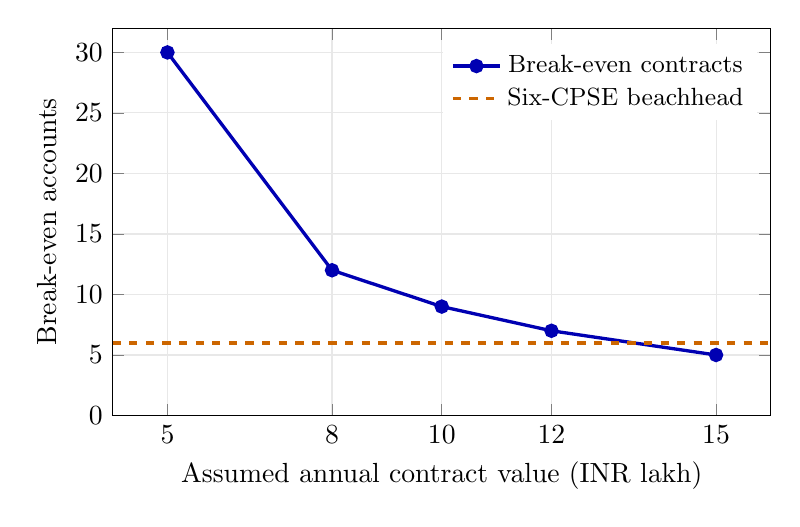
\begin{tikzpicture}
\begin{axis}[
  width=.82\textwidth,height=65mm,
  xlabel={Assumed annual contract value (INR lakh)},
  ylabel={Break-even accounts},
  xmin=4,xmax=16,ymin=0,ymax=32,
  xtick={5,8,10,12,15},
  ytick={0,5,...,30},
  grid=both,grid style={gray!18},
  legend style={draw=none,at={(.98,.96)},anchor=north east,font=\small},
  ]
\addplot[very thick,blue!70!black,mark=*,mark options={fill=blue!70!black}]
coordinates {(5,30) (8,12) (10,9) (12,7) (15,5)};
\addlegendentry{Break-even contracts}
\addplot[dashed,very thick,orange!80!black,domain=4:16]{6};
\addlegendentry{Six-CPSE beachhead}
\end{axis}
\end{tikzpicture}
\caption{The required number of customers falls as assumed ACV rises. The horizontal line is the maximum of the six-CPSE beachhead if every organization buys independently.}
\label{fig:breakeven}
\end{figure}

The result is also sensitive to direct integration cost. At \(P=10\), if customer delivery costs \inr2, \inr3, or \inr5\lac{} annually, the annual threshold is respectively 8, 9, or 12 accounts. Fixed cost matters: with \(P=10\), \(v=3\), and fixed cash cost of \inr40, \inr60, or \inr90\lac{}, break-even requires 6, 9, or 13 accounts. No single point estimate should be presented without these ranges.

\section{Three-year conditional cash illustration}

The following is a deliberately explicit \emph{scenario}, not a sales forecast. Suppose a one-time \inr5\lac{} setup outflow at time zero; annual fixed cash cost remains \inr60\lac{} (including the conservatively spent or committed contingency); price and direct cost remain \inr10 and \inr3\lac{} per customer; paying customers number one, three, and nine in years 1--3; contracts are billed and collected in their respective years. This assumes substantial expansion outside the six-refiner beachhead by year 3. It also assumes no annual price inflation, churn, delayed procurement, or receivables.

\begin{table}[htbp]
\centering
\caption{Conditional three-year cashflow (INR lakh). Parentheses indicate cash deficits. Customer counts are hypothetical, not a pipeline.}
\label{tab:cashflow}
\small
\begin{tabular}{@{}lrrrr@{}}
\toprule
 & Setup, \(t=0\) & Year 1 & Year 2 & Year 3\\
\midrule
Paying accounts & --- & 1 & 3 & 9\\
Receipts \(=10N\) & 0 & 10 & 30 & 90\\
Direct customer cost \(=3N\) & 0 & (3) & (9) & (27)\\
Fixed annual cash cost & 0 & (60) & (60) & (60)\\
One-time setup & (5) & 0 & 0 & 0\\
\midrule
Annual net cash & \textbf{(5)} & \textbf{(53)} & \textbf{(39)} & \textbf{3}\\
Cumulative cash & \textbf{(5)} & \textbf{(58)} & \textbf{(97)} & \textbf{(94)}\\
\bottomrule
\end{tabular}
\end{table}

\begin{figure}[htbp]
\centering
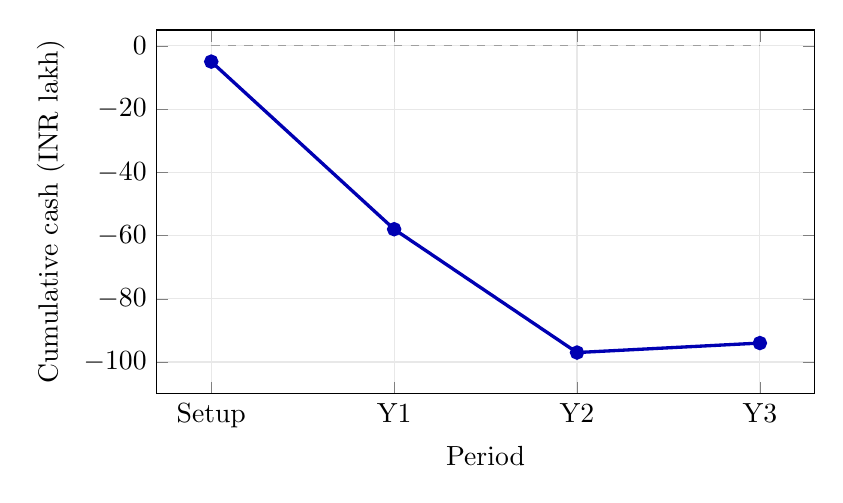
\begin{tikzpicture}
\begin{axis}[
  width=.82\textwidth,height=62mm,
  xlabel={Period},
  ylabel={Cumulative cash (INR lakh)},
  symbolic x coords={Setup,Y1,Y2,Y3},
  xtick=data,ymin=-110,ymax=5,
  ytick={-100,-80,...,0},
  grid=major,grid style={gray!18},
  ]
\addplot[very thick,blue!70!black,mark=*,mark options={fill=blue!70!black}]
coordinates {(Setup,-5) (Y1,-58) (Y2,-97) (Y3,-94)};
\addplot[dashed,gray!75] coordinates {(Setup,0) (Y3,0)};
\end{axis}
\end{tikzpicture}
\caption{A year-3 operating break-even does not recover earlier investment. Under the stated assumptions, cumulative cash remains \(-\inr94\lac{}\) after three years.}
\label{fig:cash}
\end{figure}

Annual operating break-even and payback are different. In this illustration, year 3's nine accounts produce only \inr3\lac{} positive cash, while cumulative cash remains negative \inr94\lac{}. To recover that balance in a single additional year at unchanged costs and price would require \((94+60)/7=22\) whole customer contracts in year 4. That is far beyond the six-refiner beachhead and unvalidated. A research grant, procurement partnership, licensing rights in a larger sector, a cheaper delivery process, or a higher contract price could change the economics; no such funding or customers are assumed here.

\section{A measured buyer value test}

A solver purchase should be evaluated against \emph{operational decisions}, not license prices alone. For each consenting industrial partner, capture a portfolio of real models and define the target deadline, feasible-solution requirements, optimality-gap target, objective units, and fallback process before running the new engine. Then run the candidate and a strong available baseline at matched hardware, threads, wall time, model input, and verification tolerance. An independent checker should verify every returned point against the original model. Infeasible and time-limited statuses need separate accounting.

The business metric should be computed only when the model's objective has an approved mapping to a real decision and financial period. For a refinery blend, a modelled profit difference is not automatically booked profit: yields, prices, inventories, process limits, and operating constraints must be checked by domain owners. A recommended pilot would report:
\begin{itemize}
  \item Technical measures: solution availability, primal feasibility, objective, bound and gap, wall time, memory, reproducibility, and failure count.
  \item Decision measures: which planned actions change, whether operators would accept them, and whether performance persists under representative input perturbations.
  \item Economic measures: independently approved annualized value, integration cost, recurring support and compute, and the cost of a wrong or delayed answer.
\end{itemize}

The project currently has public benchmark and literature/synthetic demonstration data rather than an approved MRPL production model. Its current solver limitations and version-specific results belong in the technical paper; the market paper uses them as a qualification gate, not as a rupee benefit estimate. Even a feasible model solution must meet the customer's operational acceptance criteria before benefit can be claimed.

\section{Procurement, ownership, and commercialization gates}

The first likely route is a controlled, paid pilot, with a clearly bounded model family and service period. Before presenting a commercial proposal, the team should establish ownership and licensing rights for the solver; a bill of materials and dependency license audit; a supported platform and security baseline; model and data confidentiality terms; a reproducible performance and failure-reporting procedure; customer support obligations; and a buyer-specific comparison with alternatives. Any public procurement preference or sovereign-technology claim should be checked against the actual tender and prevailing rules rather than assumed to guarantee an award.

The addressable-account funnel should be maintained as a named evidence ledger, not a slide-only multiplier. A prospect advances from named to qualified only when the use case, data, sponsor, decision deadline, buying entity, budget, incumbent alternative, and pilot acceptance criteria are recorded. A prospect counts toward \emph{realized} SOM only after an executed paid contract; before that it remains the prospective scenario. This avoids silently treating a PPAC refinery facility row, its parent CPSE, and a subsidiary as three customers.

\begin{table}[htbp]
\centering
\caption{Evidence required to replace illustrative inputs with an investment-grade case.}
\label{tab:gates}
\small
\begin{tabularx}{\textwidth}{@{}p{31mm}X p{36mm}@{}}
\toprule
Claim to support & Required evidence & Present status\\
\midrule
Eligible accounts & Named list with legal entity, model owner, recurring optimization use case, and decision authority & Sector and refinery names identified; no demand survey\\
Annual price \(P\) & Real priced proposals, paid pilots, or procurement comparators of equivalent scope & \inr5--15\lac{} is a scenario range\\
Direct cost \(v\) & Recorded engineering hours, cloud invoices, support tickets, and deployment effort for pilots & \inr3\lac{} is an assumption\\
Annual fixed cost \(F\) & Staffing plan, signed offers, cloud/hardware quotations, support policy & \inr60\lac{} is a planning budget\\
Buyer ROI & Authorized industrial model, incumbent comparison, independent solution checking, domain approval, and decision-value accounting & No MRPL operating-data ROI demonstrated\\
National expansion & Disjoint organization-level market list across CPSE, state, and private sectors; avoid site and company duplication & No audited India-wide buyer database\\
\bottomrule
\end{tabularx}
\end{table}

\section{Limitations and decision}

This analysis is intentionally narrower than a commercial market report. Its observations are counts published by Indian public agencies and price/license terms published by solver vendors. There is no primary survey of Indian solver procurement, no India deployment quote for CPLEX or Gurobi, no signed order, no customer adoption probability, and no actual project expenditure ledger in the reviewed folder. The solver's benchmark portfolio cannot establish willingness to pay. The figures should not be presented as current revenue, national software TAM, or guaranteed savings.

Under the illustrative \inr10\lac{} ACV and \inr60\lac{} fixed annual cash budget, nine paying accounts cover annual running costs. Six sector refinery CPSEs offer a coherent initial technical and commercial focus but cannot alone support this assumed team cost at that price. The next economic experiment is therefore a scoped paid pilot and a named 97-enterprise qualification exercise, paired with real integration times and comparable deployment quotes. If measured costs or buyer prices differ, the formulas and charts in this paper can be updated directly. Until that evidence exists, the strongest honest conclusion is that a domestic solver could have strategic and commercial value, while its current INR opportunity and payback remain conditional.

\section*{Reproducibility note}

All figures and tables were generated from the counts and assumptions printed here. The arithmetic is: \(291\times10/100=29.1\) crore; half-up \(\lfloor97q+\tfrac12\rfloor\) equals 24, 49, and 73 for \(q=0.25,0.50,0.75\); \(6\times10=60\) lakh for the CPSE-refinery beachhead; \(N_{\mathrm{break-even}}=\lceil60/(P-3)\rceil\); and the cash scenario uses \(N=(1,3,9)\). No external commercial market-size estimate or hidden spreadsheet drives the numbers. Source pages were accessed on 26 September 2026. PPAC's capacity table states 1 April 2026 and displayed an update date of 25 September 2026 when checked.

\begin{thebibliography}{99}
\bibitem{dpe2025}
Department of Public Enterprises, Ministry of Finance, Government of India,
\emph{Public Enterprises Survey 2024--25}, published December 2025.
The report states 291 operating CPSEs and 97 in manufacturing, processing, and generation.
\url{https://reports-pesurvey.dpe.gov.in/pesurveyreports/FY2024-25/PESurveyReportFY2024-25_English.pdf}.
Accessed 26 September 2026.

\bibitem{dpeappendix}
Department of Public Enterprises, Ministry of Finance, Government of India,
\emph{Public Enterprises Survey 2024--25}, Appendix II: Operating CPSEs under Different Sectors/Cognate Groups.
The petroleum-refinery/marketing list contains BPCL, CPCL, HPCL, IOCL, MRPL, and NRL within manufacturing, processing, and generation; ONGC is classified under crude-oil mining.
\url{https://reports-pesurvey.dpe.gov.in/pesurveyreports/FY2024-25/APPENDIX-II.pdf}.
Accessed 26 September 2026.

\bibitem{ppac2026}
Petroleum Planning \& Analysis Cell, Ministry of Petroleum and Natural Gas, Government of India,
Installed Refining Capacity, table dated 1 April 2026.
\url{https://ppac.gov.in/infrastructure/installed-refinery-capacity}.
Accessed 26 September 2026.

\bibitem{hrrl2026}
Press Information Bureau, Ministry of Petroleum and Natural Gas, Government of India,
Cabinet approval concerning HPCL Rajasthan Refinery Limited, 8 April 2026; scheduled commercial operation date 1 July 2026.
\url{https://www.pib.gov.in/PressReleasePage.aspx?PRID=2250055&lang=2&reg=3}.
Accessed 26 September 2026.

\bibitem{asi2024}
Ministry of Statistics and Programme Implementation, Government of India,
Annual Survey of Industries, 2023--24, released 2025.
\url{https://www.mospi.gov.in/themes/product/65--}.
Accessed 26 September 2026.

\bibitem{asisummary}
Ministry of Statistics and Programme Implementation, Government of India,
\emph{Summary Results for Factory Sector: Annual Survey of Industries 2023--24}, Section 3.1.2.
\url{https://new.mospi.gov.in/uploads/publications_reports/publications_reports1759229789833_2b8ed8ad-314e-46b7-b123-b08cb17f1233_ASI_Summary_Results_2023-24C.pdf}.
Accessed 26 September 2026.

\bibitem{ibmprice}
IBM,
IBM ILOG CPLEX Optimization Studio: pricing and licensing options.
\url{https://www.ibm.com/products/ilog-cplex-optimization-studio/pricing}.
Accessed 26 September 2026.

\bibitem{gurobiprice}
Gurobi Optimization,
Gurobi pricing and licensing.
\url{https://www.gurobi.com/product/pricing-and-licensing}.
Accessed 26 September 2026.

\bibitem{highs}
HiGHS Optimization,
HiGHS: linear optimization software, official project repository and license.
\url{https://github.com/ERGO-Code/HiGHS}.
Accessed 26 September 2026.

\bibitem{scip}
SCIP Optimization Suite,
License, official project site.
\url{https://www.scipopt.org/}.
Accessed 26 September 2026.
\end{thebibliography}

\end{document}
